\documentclass[border=10pt]{standalone}
\usepackage{tikz}
\usetikzlibrary{positioning}
\tikzset{vertex/.style = {font = \sffamily\bfseries, text = white,
      shape = circle, ball color = blue}}
\tikzset{bridge/.style = {thick, double = yellow,
      double distance = 1pt}}
\tikzset{number/.style = {font = \sffamily\bfseries, text = white,
      draw,fill = red}}
\begin{document}
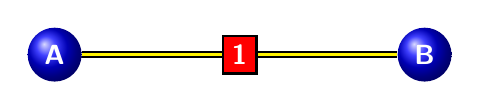
\begin{tikzpicture}
  \node[vertex] (A) {A};
  \node[vertex, right = 4 cm of A] (B) {B};
  \draw (A) edge[bridge] node [number] {1} (B);
  \end{tikzpicture}
\end{document}
